When designing maps, there is one difference to be made: designing maps for print versus the internet. For the first case, the design is for map readers, whereas for the latter case, it is for map users. The difference between readers and users lays in the interaction. This chapter focuses on map designed for the internet and therefore allowing a lot more interaction. Users do not only interact but also manipulate web maps. Interaction for print maps would be moving a paper map closer or further away to one's eyes, or trim specific parts with scissors and so forth. The weakness of this kind of interaction is that the data on the map stays the same. However, zooming, selecting and moving a map on the internet actually allows for adapting the data shown \iacite{Muehlenhaus2014}.

As already mentioned in chapter \ref{s:definitions-types} on page \pageref{s:definitions-types}, \citeauthor{Shneiderman1996} published an often cited mantra \iacite{Shneiderman1996}:
\begin{quote}
Overview first, zoom and filter, then details on demand.
\end{quote}

% MISSING BOOK: Information Visualization: Design for Interaction Spence 2007
% This mantra can also be used as a guideline for creating web maps with interaction.
% % Spence2007
% introduces a so called action cycle, which models an interactive exploration process of data. Small datasets, as well as complex and dynamic data can make use of this process in order to properly implement and integrate interaction.

% TODO - CHECK IF ENOUGH WORDS

The first part of this chapter will introduce some basic interaction methods and concepts. The second part will build upon the knowledge of the first part and maps the basic concepts to today's implementations with the focus on interaction with thematic maps.

\subsubsection{Overview First, Focus + Context}
A natural way according to the mantra presented by \citeauthor{Shneiderman1996} to visualise a dataset is to start with an overview. This supports the user's understanding of the complexity and size of the whole dataset. However giving an overview first is also dependant on the dataset. Imagine a \ac{GIS} like OpenStreetMap\footnote{See \href{https://www.openstreetmap.org}{https://www.openstreetmap.org}} would show random location, e.g. a valley with a lot of detail as a starting point. There are two contrary use cases where such a starting point would make sense or not.
\begin{enumerate}
\item If the dataset the map is based on only contains data of that specific ``random'' valley shown, it definitely makes sense to only show that valley. The dataset does not contain information about all valleys, therefore making it unnecessary to show the whole map of the earth as an overview first.
\item The use case mentioned already, implicitly explains a bad use case of a random starting point. If a dataset inheres structure, like a whole map of the world, it is not useful to start at a specific location, therefore showing an overview of the earth first makes more sense.
\end{enumerate}

Focus and context describes a concept that puts a specific part of dataset, called subset, in focus while still showing an overview of the other part. One example implementation of this concept are fisheye views, originally developed by \citeauthor{Furnas:1986} \iacite{Furnas:1986}. Figure \ref{fig:focus} on page \pageref{fig:focus} shows a modern implementation of the focus and context concept based on a fisheye view. The focus in this Figure is set somewhere between the blue and orange circle in the middle of the Figure. This part is magnified as one can see on the circle size, while the ones further away are smaller and a little distorted.

\begin{figure}[!htb]
\centering
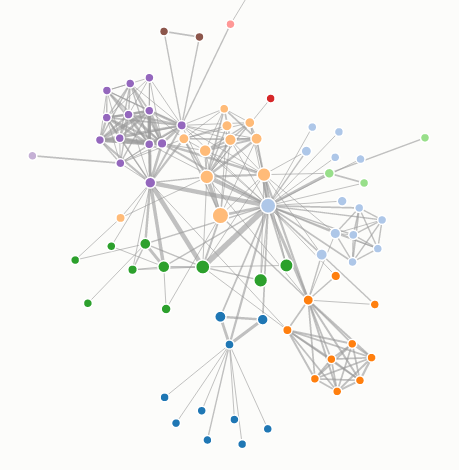
\includegraphics[height=5cm,keepaspectratio]{images/methods/interaction/focus.png}
\caption[
    The focus and context concept based implemented with a fisheye view, Urldate: 07.2016 \newline
    \small\texttt{\url{https://bost.ocks.org/mike/fisheye/}}.
]{The focus and context concept implemented with a fisheye view. The blue node in the center of the Figure and the yellow node left to it are bigger compared to the other ones. This is due to the magnification of this part.}
\label{fig:focus}
\end{figure}

\citeauthor{Kosara2003} categorise the aforementioned method as distortion-oriented \iacite{Kosara2003}. Other techniques they list are summarised below:
\newpage
\begin{description}
\item[Overview methods] show the context in a separate layer in the same place \iacite{Kosara2003}.
\item[Filtering] shows additional information of particular subparts e.g. with a magic lens. They provide an object of any shape that can move freely. The area it covers is shown with more information \iacite{Bier:1993}.
\item[In-Place techniques] are similar to filtering without the requirement of a lens. The implementation of the technique points out information to the user, e.g. by highlighting. The program can also take the initiative and point the user to interesting data \iacite{Kosara2003}.
\end{description}


\subsubsection{Details on Demand}
Showing detailed information upon interaction on a dot map based on a dataset with 10000 data items describes the concept of showing details on demand. It would be infeasible to show details on all entries, as the screen-space is limited. Even with unlimited screen-space it, would drastically worsen the readability of the map. \citeauthor{Ahlberg:1996} explains one possible way of implementing this concept. His approach is to only show objects that match certain criteria and are therefore likely of interest to the user. However, the user needs to start this task first with some kind of interaction, e.g. clicking on a visual object of a specific type. The additional information is then shown in a pop-up window \iacite{Ahlberg:1996}.



\subsubsection{Multiple Views, Linking \& Brushing}
\label{s:linking-brushing}
Multiple view systems are defined by using several views on the same dataset, but with different aspects of it for each visualization. Practical applications of all kinds make use of such a system, e.g. \ac{CAD} and \ac{GIS}. Even though the possibility of using multiple views on the same dataset is trivial, the implementation and necessary amount of interaction is not \iacite{Kosara2003}.

\citeauthor{Baldonado2000} present four design rules wheter or not multiple view systems are appropriate for the specific task \iacite{Baldonado2000}:

\begin{enumerate}

\ditem{Diversity} \hfill \\
If the given dataset consists of attributes with different types, multiple levels of abstraction, and so forth, a multiple view system can be created. A single view would be overloaded with the given dataset because of the significant cognitive overhead created. The user would need to simultaneously comprehend and assimilate a multitude of diverse data.

\ditem{Complementarity} \hfill \\
Multiple view systems support visual comparability. They should be used if showing correlations and/or disparities is important, because they leverage multiple perceptual capabilities to improve understanding of relations among views.

\ditem{Decomposition} \hfill \\
Showing different attributes at the same time provides insight in different dimensions. This rule is related to the "divide and conquer" principle: the amount of data a user needs to consider at one time is reduced, thus aiding memory.

\ditem{Parsimony} \hfill \\
Multiple views build upon the cost of switching context and increasing complexity. The learning cost of a user, aswell as computational and display space costs of several views must be justifiable.

\end{enumerate}

Multiple view systems are often used for focus and zoom, e.g. for showing the focus and contex in seperate windows. \citeauthor{Robert:1998} describe a system based on this concept \iacite{Robert:1998}.

\citeauthor{Martin:1995} describe brushing as the process of selecting specific data items or groups of items to highlight them \iacite{Martin:1995}. Usually this process is initiated by directly interacting with the view using the mouse. Two possible manual interactions are opening a rectangular region of interest or clicking on a specific data items. It can also be accomplished without interacting with the visualization itself by using sliders, select-boxes or even complex means like selecting a cluster \iacite{Kosara2003}.

However, using the brushing technique is not sufficient when exploring complex data efficiently. Linking describes the concept of exchanging information about which points are brushed. This concept is essential when using brushing and multiple view systems together. With this combination, a user can easily see the same points brushed in different views on the data \iacite{Kosara2003}.



\subsubsection{Animations and Transitions}
In order to understand transition referring to visualizations, it is important to point out the difference between transition and animation. Even though these two terms are often substituting each other, they follow two different concepts \iacite{Muehlenhaus2014}:

According to the Merriam Webster Online Dictionary\footnote{See \href{http://www.merriam-webster.com/}{Merriam Webster Dictionary}} an animation is a way of making a movie by using a series of drawings, computer graphics or photographs that are slightly different from one another and that when viewed quickly one after another create the appearance of movement. Transition, however, is a movement, development, or evolution from one form, stage, or style to another.

With these definitions, it is easy to distinguish the two terms. Animation is the process of making any kind of movement visible to a user, whereas transitions in visualizations make use of animations to show e.g. the change of visual appearance.

\citeauthor{Thrower1959} was the first one to combine the research fields of cartography with animation. He describes the process of bringing e.g. population growth with animation on a map \iacite{Thrower1959}. However, animated cartography remained a bit of an oddity that was experimented with. This fact could not be changed even with the rise of the household \ac{PC}. Nonetheless, the mass adoption of the internet could counteract the rare usage of map animation \iacite{Muehlenhaus2014}.

This chapter furthermore describes considerations when designing animated maps. Animation can basicly be broken down into two broad types:

\begin{enumerate}
\ditem{Stop-Frame Animation} \hfill \\
This type of animation is also known as stop motion. Every frame of this type of animation is designed separately. After many pictures and movements are made, all pictures are in the order they were taken. The rate of change for each picture heavily influences the cognition of the animation \iacite{Faroudja1991}.
\ditem{Tweening} \hfill \\
    This term bears its name from the word "betweening". It describes the process of interpolating movement between key frames, thus creating smoother animations compared to the stop-frame method \iacite{Muehlenhaus2014}.
\end{enumerate}

\citeauthor{DiBiase1992} identified three new visual variables dealing specifically with animation \iacite{DiBiase1992}:

\begin{enumerate}

\ditem{Duration} defines the temporal length of how long a particular frame in an animation is shown. Imagine a dataset containing decennial census of population data and an animation set to 24 frames per second. To give each map user the ability to conceive each decade, it is needed to show it at least for some seconds. For the sake of convenience a duration of 2 seconds is assumed to be enough. Therefore, it is needed to show each decennial census data for 48 frames, resulting in a 2 second duration \iacite{Muehlenhaus2014}.

\ditem{Rate of Change} represents how quickly an image is morphed into the next attribute. In general, it denotes the magnitude of an attribute divided by the duration. This basically means, that it is needed to know how much the animated image being represented changes from frame to frame \iacite{Muehlenhaus2014}.

\ditem{Order}
Rather than animating data in the order they are given, they can be reorganized first by a specific attribute. For example, one could show all countries with a high population first, before showing small ones \iacite{Muehlenhaus2014}.

\end{enumerate}

\citeauthor{Muehlenhaus2014} also mentions differnt types of map animations. He says weather forecasts are the most common use case for map animations. Thus deriving the term temporal animation for this kind of animation seems appropriate. Albeit showing change over time seems trivial, people do not always interpret the resulting animation accurately. He suggests the use of temporal animations for showing broad patterns of change in a dataset. However, the animation should either show broad changes in a small scale or detailed changes in a large scale. This heavily impacts the user's perception and interpretation of the animation, including "change blindness". This means, that obvious changes in a map are missed due to focusing something else in the map. In order to combat the problem of change blindness, he \citeauthor{Muehlenhaus2014} names three different design principles \iacite{Muehlenhaus2014}:

\begin{enumerate}

\item \textbf{Animation duration} should be kept short in order to not overwhelm a user's short-term memory. Temporal animations should not take longer than 30 seconds to a minute, especially when showing changes in data, which are not narrative in nature. If this principle is ignored, data retention will be nullified \iacite{Muehlenhaus2014}.

\item \textbf{Data simplification} denotes the amount of animated attributes used. Showing more than four attributes in an animation results in visual overstimulation \iacite{Ware2008}.

\item \textbf{Control} needs to be given to the user. This can be achieved in many ways, e.g. by providing a pause or play button for an animation \iacite{Muehlenhaus2014}.

\end{enumerate}

Another type of animation \citeauthor{Muehlenhaus2014} mentions is the so called zoom animation. This type basically follows the main visual information seeking mantra of \citeauthor{Shneiderman1996}. If the purpose of an animation is to show a specific part of the data, it should start off by giving an overview. The animation is either started programmatically or manually and animates the focus to a specific part of the data. Control can ge given to the user in form of freely moving around in the map or providing zoom buttons.

However, the mentioned types of animations are only based on a single visualization. This thesis will use animation in a transition of one type of map visualization to another. First, this should help to understand how the map is created. Second, some map visualizations are based on aggregations and therefore, the animation should show if this aggregation is understandable and interpretable.

